\documentclass[12pt,fleqn]{article}\usepackage{../common}
\begin{document}
Ders 19

Konumuz vektor alanlari (vector fields) ve cizgi entegralleri (line
integrals). Bundan onceki derslerde cift entegral (double integral)
konusunu isledik, fakat o tur entegraller cizgi entegrallerinden tamamen
farklidir, yani bu dersi takip ederken cift entegraller ile baglantilari
dusunmemek daha iyi olur, kafalar karismasin. 

Vektor Alanlari

Vektor alanlari bir vektordurler aslinda, diyelim ki $\vec{F}$

\[ \vec{F} = M\hat{i} + N\vec{j} \]

Farkli olan $M,N$ kendilerinin $x,y$'nin bir fonksiyonu olmalaridir. Bu
demektir ki kordinat sistemindeki her $x,y$ kombinasyonu icin degisik bir
vektor olacaktir. Bir misir tarlasinda her noktada misir vardir, vektor
alaninda her noktada bir vektor vardir [hoca bu analojiyi misirlar uzun,
yonleri olan seyler oldugu icin kullaniyor herhalde]. Daha once
$\vec{r}(t)$ baglaminda $t$ degiskenine bagliligi gorduk, fakat o tek
degisken idi, zaten bir egriyi vektor ile temsil etmek icin oyle olmasi
gerekiyordu, burada birden fazla degisken $x,y$'ye bagimlilik var. 

Bu kavram bir sivi, bir ruzgar icindeki akis vektorlerini temsil etmek icin
kullanilabilir mesela. Ya da kuvvet alani (force field) kavrami -- bu
kavram Star Wars filminden bir kavram degil. Yeryuzunde elimizde bir cismi
herhangi bir yerde tuttugumuzda onun uzerinde etki eden bir kuvvet vektoru
var, bu vektor her noktada degisik, ve tum bu vektorlerin toplami bir
kuvvet alani olusturuyorlar, ki bu alan bir vektor alanidir. 

Biz bu derste konuya pur matematiksel olarak bakiyoruz, sadece arka
plandaki bu fiziksel baglantiyi motivasyon acisindan aklimizda
tutabiliriz. 

Once cizimden baslayalim

Ornek

\[ \vec{F} = 2\hat{i} + \hat{j} \]

Tam $x,y$'ye baglantidan bahsetmistik, baglantisiz bir tane verdik! Ama
ornegi soyle gorebiliriz, bu alan her $x,y$ icin ayni vektore sahip. Yani
yine $x,y$'yi merkez alarak dusunuyoruz, sadece vektorun her noktada ayni
oldugunu soylemis oluyoruz.

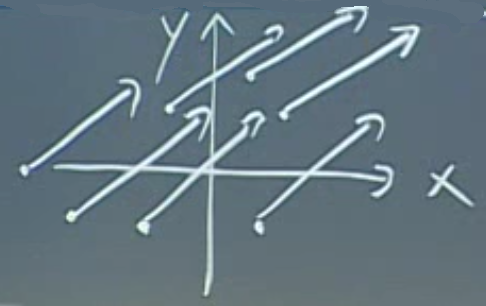
\includegraphics[height=4cm]{19_1.png}

Ornek

\[ \vec{F} = x\hat{i} \]

Y-ekseni uzerinde, yani $x$'in sifir oldugu noktada (zaten hic $y$ yok)
vektor sifir buyuklugunde. Diger noktalarda vektor yatay, $x$ buyudukce, ya
a eksi yonde kuculdukce, saga ya da sola dogru vektorun buyuklugu de
degisecek.

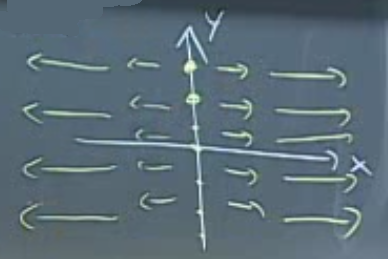
\includegraphics[height=4cm]{19_2.png}

Aslinda bu tur cizimleri cogunlukla bilgisayara yaptiriyoruz, ama kabaca
vektor alanlarinin neye benzedigini hayal edebilmek ise yariyor. 

Ornek

\[ \vec{F} = x\hat{i} + y\hat{j} \]

Bu alanin ilginc bir geometrik sonucu var.  Orijinden herhangi bir noktaya
cizilebilecek bir vektoru (... ile belirtiliyor) alip, kopyalarsak, bu
kopyayi o noktadan baslayacak sekilde yerlestirirsek, dogru sonucu elde
etmis oluruz.

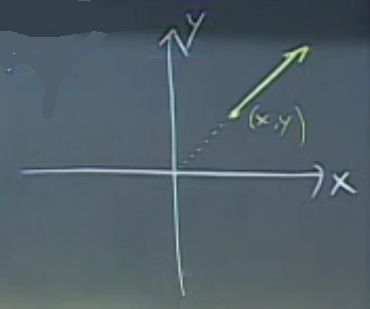
\includegraphics[height=4cm]{19_3.png}

Hepsini cizince su sekil ortaya cikiyor. 

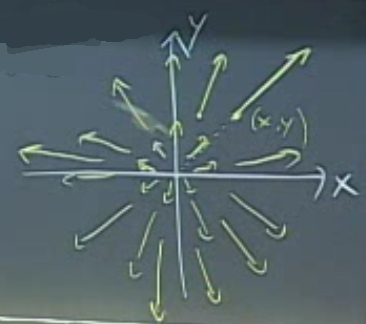
\includegraphics[height=4cm]{19_4.png}

Bu cizim teknigi bu ornekte ise yaradi cunku $x,y$ hem vektor buyuklugunu,
hem de alan baglaminda onun baslangic noktasini belirliyor. 

Ornek

\[ \vec{F} = -y\hat{i} + x\hat{j} \]

Yine orijinden baslama numarasini dusunursekm simdi elimizde $<-y,x>$
vektoru var, acaba bu vektor $<x,y>$ gore nasil bir vektor? 

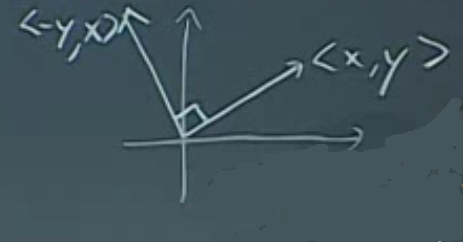
\includegraphics[height=2cm]{19_5.png}

Bu iki vektorun arasinda 90 derece vardir. O zaman bu $<x,y>$'ye dik olan
kopyayi almamiz lazim, ve onu $x,y$'den baslatmamiz lazim. 

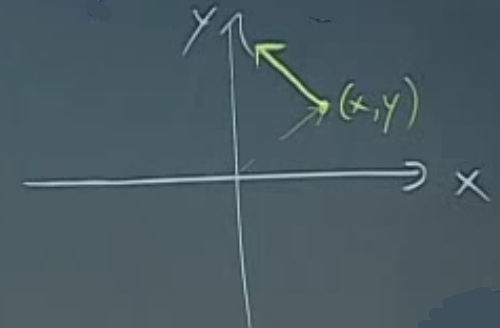
\includegraphics[height=4cm]{19_6.png}

Hepsini cizersek

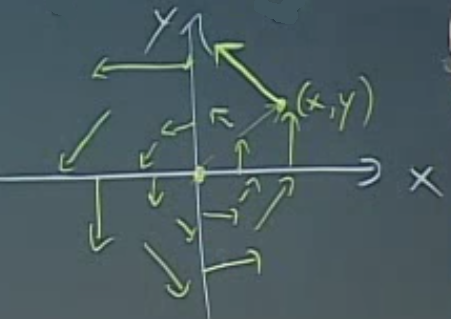
\includegraphics[height=4cm]{19_7.png}

Bu alan mesela orijin etrafinda her yuvarlakta sabit hizda bir akisi olan
bir siviyi temsil ediyor olabilir. Yani vektor alani bir hiz alani
(velocity field) olabilir. Ilginc sorulardan biri, sivi icindeki bir
parcacigin halkalarin birinde tam bir atmasinin ne kadar zaman
alacagi. Cevap $2\pi$ cunku halkanin uzunlugu $2\pi \cdot r$, yani $2\pi$
carpi yaricap (radius). Bu cevap birim acisal hiz (unit angular velocity),
1 radyan / zaman. Hizin buyuklugu bir halka icinde sabit, cunku hizin
buyuklugu demek vektorun buyuklugu demek, eger halkayi biz sectiysek, o
halkanin orijinden uzakligi ayni olacaktir, bu uzakligin kopyasi da ayni
buyuklukte olacaktir. 

Kuvvet alanlarina gelelim, yani simdi vektor alandaki vektorler kuvvetleri
temsil edecekler. Simdi su senaryoyu dusunelim. Bir parcacigin uzerine bir
kuvvet uygulaniyor ve bu parcacik bir seyahat cizgisi uzerinde
ilerliyor. Fizikten bilindigi gibi kuvvetin yaptigi ``is (work)'' kuvvetin
o kuvvetin sayesinde ne kadar yer degisikligi oldugunun vektoru
(displacement vector) ile noktasal carpimina esittir. Eger gidisat duz
olursa, ve kuvvet sabitse bu hesap basitce yapilabilir, ama daha cetrefil
bir gidisat takip ediliyorsa ve kuvvet o sirada surekli degisiyorsa, o
zaman uzerinden entegrasyon yapmamiz gerekir.

Is ve Cizgi Entegrali

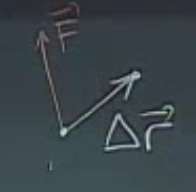
\includegraphics[height=2cm]{19_8.png}

\[ W = (kuvvet)\cdot(mesafe) = \vec{F}\cdot\Delta\vec{r} \]

$W$ yapilan is (work)'i temsil ediyor. 

Fakat senaryomuzda demistik ki gidisat karmasik ve guc surekli
degisiyor.

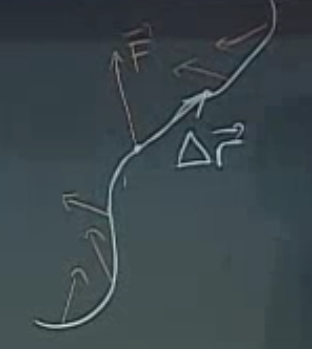
\includegraphics[height=4cm]{19_9.png}

O zaman is hesabini yapmak icin gidisati ufak parcalara ayirmaliyim, o
parcalar icin carpimi yapip sonuclari toplamaliyim. Parcalar olabilecegi
kadar ufak olmali tabii ki, bu ne demektir? Bir entegral demektir. Yani

Bir gidisat $C$ uzerinde yapilan is 

\[ W = \int_C \vec{F} \cdot d\vec{r} \]

Notasyonun hesapsal anlamina bakalim simdi. Soyle gorebiliriz

\[ = \lim_{\Delta r_i \to 0} \sum_i  \vec{F} \cdot \Delta\vec{r}_i\]

\[ = 
\lim_{\Delta t \to 0} \sum_i  
\vec{F} \cdot \bigg( \frac{\Delta\vec{r}}{\Delta t} \Delta t 
\bigg)
\]

Aslinda hem bolume, hem bolene $\Delta t$ ekleyerek hic bir sey
degistirmedik, ama yeni ortaya cikan terim $\Delta\vec{r} / \Delta t$ hiz
vektoru $d\vec{r}/dt$'ye esit. Limitin $\Delta t$'ye donustugune dikkat.

Yani ilk bastaki entegralimizi su sekilde hesaplayabiliriz

\[ = \int_{t_1}^{t_2} \vec{F} \cdot \frac{d\vec{r}}{dt} dt \]

Ornek

Su kuvvetin

\[ \vec{F} = -y\hat{i} + x\hat{j} \]

Su parametrik egri $C$ uzerinde

\[ x = t  \]

\[ y = t^2 \]

\[ 0 \le t \le 1 \]

yaptigi isi hesapla. 

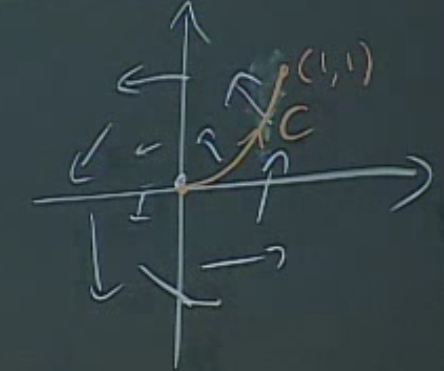
\includegraphics[height=3cm]{19_10.png}

Bu arada, ``$C$'yi nereden buldun?'' diye bir soru gelebilir, bu yanlis bir
soru. $C$'yi bulmadik, o bize sorunun icinde verildi, yani elimizdeki veri
bu. Kuvvet alani ve egri tamamen ayri yerlerden, ayri sekilde tanimlanmis
olabilir. 

\[ \int_C \vec{F} \cdot d\vec{r} 
= \int_{0}^{1} \vec{F} \cdot \frac{d\vec{r}}{dt} dt 
\]

$\vec{F}$ nedir? 

\[ \vec{F} = <-y,x> = <-t^2,t> \]

Hiz nedir? 

\[ dx/dt = 1 \]

\[ dy/dt = 2t \]

O zaman 

\[ W = \int_{0}^{1}  <-t^2,t>\cdot<1,2t>dt \]

\[ = \int_{0}^{1} (-t^2 + 2t^2)dt\]

\[ = \int_{0}^{1} t^2dt = \frac{1}{3} \]


Baska Bir Yol

Vektor alanimizin bilesenlerinin

\[ \vec{F} = <M,N> \]

oldugunu dusunelim, ve

\[ d\vec{r} = <dx, dy> \]

Cunku $\vec{r}$ parametrize edilmis bir vektor, ve bilesenleri $x,y$
seklinde. O zaman

\[  \vec{F} \cdot d\vec{r}  = M dx + N dy
\]

olacaktir. Bu esitlik uzerinden problemlerin cogunlukla su sekilde
yazildigini gorursunuz

\[  \int_C \vec{F} \cdot d\vec{r}  = \int_C M dx + N dy\]

Esitligin sagindaki vektor alani degil artik, ama aslinda asagi yukari ayni
seyler. Yani aradaki fark bir fonksiyonun gradyani ile kismi
diferansiyelleri arasindaki iliskiye benziyor. Notasyon farkli, ama aslinda
ayni icerige sahipler. 

Peki bu yeni formdaki cizgi entegralini nasil hesaplayalim? Hem $M$ hem $N$
icinde $x,y$ var, eger entegrali sadece $dx$, sadece $dy$ icin alirsak yine
$y$'ler, $x$'ler ortaya cikacak, fakat biz bunu istemiyoruz, biz tek bir
sayi istiyoruz. Buradaki puf nokta su, egri boyunca $x,y$ birbiriyle
baglantili. Yani $M,N$ iceren bir formulu entegre ediyor olabiliriz, ama
$C$ boyunca aslinda sadece tek bir parametre var. Bu tek degiskn $x$
olabilir, $y$ olabilir, $t$ olabilir. O zaman 

Metot: $x,y$ degiskenlerini tek bir degisken baglaminda belirt. O tek degiskeni
digerlerinin yerine gecir. 

Biraz onceki ornek

\[ \int_C \vec{F} \cdot d\vec{r} 
= \int_C -y dx + x dx
\]

Her seyi yeni, tek bir degisken $t$ baglaminda belirtelim. Problem zaten
sunu vermisti

\[ x = t  \]

\[ y = t^2 \]

$dx,dy$'yi bulmak icin

\[ dx = dt \]

\[ dy = 2tdt \]

O zaman entegral suna donusur

\[ = \int_C -t^2 dt + t \cdot 2t dt\]

\[ = \int_0^1 t^2 dt = \frac{1}{3}\]


$\int_C \vec{F} \cdot d\vec{r}$ entegrali $C$'ye baglidir, parametrizasyonun nasil 
yapildigina bagli degildir. Yani hangi degiskeni istersek onu seceriz,
mesela yukaridaki ornekte 

\[ 
\left\{ \begin{array}{l}
x  = sin\theta \\
y  = sin^2\theta 
\end{array} \right.
 \]

\[ 0 \le \theta \le \frac{\pi}{2} \]

farz etmek te mumkundur. Sonra $dx,dy$ bulunurdu, bir suru trigonometrik
islemden sonra ayni sonucu bulabilirdik. Daha zor olurdu ama bulunurdu. O
zaman bir tavsiye, isimizi en kolaylastiracak parametrizasyonu kullanmak en
iyisi. Ustte en sondaki parametrizasyon pek iyi degil. 

Geometrik Yaklasim

Parametrizasyon, vs. ile her zaman bir cozume varilabilir. Fakat bazen
geometrik olarak yaklasmak cozumu daha hizlandirabiliyor. 

Vektor $\Delta \vec{r}$'yi dusunelim. 

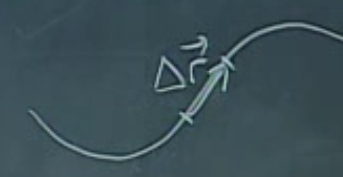
\includegraphics[height=2cm]{19_11.png}

Eger bu vektoru cok ufak alirsam, vektorun gidisata teget oldugunu
dusunebiliriz. Yani birim teget vektor ile ayni yonu gosterecek, uzunlugu
ise gidisat uzerinde alinan mesafenin ufak bir parcasi $\Delta s$ olacak. 

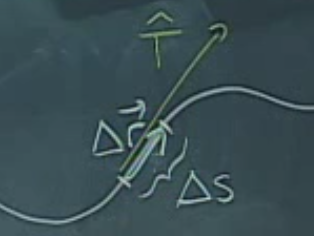
\includegraphics[height=4cm]{19_12.png}

\[ d\vec{r} = <dx, dy> \]
 
oldugu soylemistik, o zaman ayni sekilde

\[  d\vec{r} = \vec{T} \ ds \]

Dikkat esitligin sag tarafindaki noktasal carpim degil, duz carpim. Ustteki
ifadeyi su sekilde de gorebiliriz: $ds$ uzunlugunun $\vec{T}$ yonundeki
(yon sadece, cunku $\vec{T}$ birim vektor) yansimasi, bileseni.

Her seyi $dt$'ye bolunce elimize anlamli bir ifade ciktigini gorebiliyoruz

\[ \frac{d\vec{r}}{dt} = <\frac{dx}{dt}, \frac{dy}{dt}> 
= \vec{T} \ \frac{ds}{dt} 
\]

Hiz vektorunun yonu gidisatin yonune, $\vec{T}$'ye, teget.

Yani geometrik dusunerek sunu da soylemem mumkun,

\[  \int_C \vec{F} \cdot d\vec{r}  = \int_C M dx + N dy
=  \int_C \vec{F} \cdot \vec{T} ds
\]

$\vec{F} \cdot \vec{T}$'yi tek sayisal (scalar) bir nicelik olarak gorebiliriz, ki bu tek 
sayi, kuvvetin teget yonunde olan etkisi, kuvveti o yone 
``yansitinca (projection)'' ele gecen degerdir. Sonra bu yansimayi alip
tum egri boyunca entegre ediyorum. 

Ornek

$C$ = ortasi orijinde olan $a$ yaricapindaki cember, ve gidisat saat
yonunun tersi yonde.

\[ \vec{F} = x\hat{i} + y\vec{j} \]

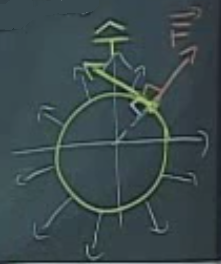
\includegraphics[height=3cm]{19_13.png}

Fizigi iyi olanlar sonucun ne olacagini tahmin edebilir, sifir olacak cunku
gidisat her zaman kuvvet vektorlerine dik. 

Yani $\vec{F} \perp \vec{T}$, o zaman $\vec{F} \cdot \vec{T} = 0$, yani

\[  \int_C \vec{F} \cdot \vec{T} ds = 0\]

Sonuc basit sekilde hesaplandi. Burada iki saat parametrizasyon
yapabilirdik, vs. ve sonuc yine ayni cikardi. 

Ornek

Ustteki ayni $C$, ama $\vec{F} = -y\hat{i} + x\hat{j}$. 

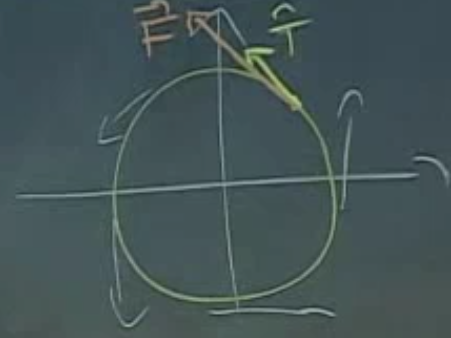
\includegraphics[height=2cm]{19_14.png}

Bu durumda her iki vektor ayni yone isaret ediyor (ama ayni buyuklukte
degiller, $\vec{T}$'nin birim vektor oldugunu unutmayalim). 

Yani $\vec{F} // \vec{T}$, o zaman $\vec{F} \cdot \vec{T} = |\vec{F}| =
a$.

Artik entegrali cok hizli sekilde hesaplayabiliriz. 

\[  \int_C \vec{F} \cdot \vec{T} ds 
=  \int_C a \ ds 
= a  \int_C ds 
= a \cdot C \textit{'nin uzunlugu }
\]

$C$'nin uzunlugu nedir? $2\pi a$. Yani ustteki entegral

\[ = 2\pi a^2 \]

Eger bu hesabi parametrizasyon ile yapsaydik? 

\[ x = acos\theta \]

\[ y = asin\theta \]

\[ 0 \le \theta \le 2\pi \]

\[ \int_C -y dx + x dy \]


\[ = \int_C -(asin\theta)(-asin\theta d\theta) + 
(acos\theta)(a cos\theta d\theta)
\]

\[ = \int_0^{2\pi} a^2 (sin^2\theta + cos^2\theta)d\theta \]

\[ = \int_0^{2\pi} a^2 d\theta \]

Ayni sonuca eristik. 

Soru 

$C$ egrisi xy duzleminde $x^2+y^2=1$ cemberi, ve yonu saat yonunun tersinde
olsun. Su cizgi entegralini hesaplayin.

\[ \int_C (2x-y)dx + (x+3y))dy \]

Parametrizasyon icin kare toplami 1 olan formulleri bulalim. Bunlar

\[ x = cos(t) \]

\[ y = sin(t) \]

\[ dx/dt = -sin(t)\]

\[ dy/dt = cos(t) \]

\[ =
\int_0^{2\pi} \bigg( 2cos(t) - sin(t) \bigg)(-sin(t))dt + 
\bigg(cos(t) + 3sin(t)\bigg)cos(t) dt
 \]

\[ = 
\int_0^{2\pi} \bigg( 
-2cos(t)sin(t) + sin^2(t) + 
cos^2(t) + 3sin(t)cos(t)
\bigg) dt
 \]

\[ = 
\int_0^{2\pi} \bigg( 
cos(t)sin(t) + 1
\bigg) dt
 \]

$cos(t)sin(t)$'nin entegrali nedir? Birbirinin turevi olan terimler carpim
olarak ayni formule olunca bir numara yapmak mumkun oluyor. Sunu 
diyebiliyoruz mesela, $u=sin(t)$ ve $du=cos(t)dt$, ve $\int u du = u^2/2$
olacagi icin, 

\[ \int cos(t)sin(t)dt = \frac{sin^2(t)}{2} \]

O zaman 

\[ = \frac{sin^2(t)}{2} + t \ \bigg|_0^{2\pi}  \]

\[ =  2\pi \]



\end{document}
